1. По теореме Виета $x_1+x_2=-\cfrac{a+3}{3},\ x_1x_2=\cfrac{a}{3}.$ Тогда $\cfrac{1}{x_1}+\cfrac{1}{x_2}=\cfrac{x_1+x_2}{x_1x_2}=
\cfrac{-\cfrac{a+3}{3}}{\cfrac{a}{3}}=-\cfrac{a+3}{a}=2,\ 2a=-a-3,\ a=-1.$ Параболу $y=3x^2+2x-1$ построим по трём точкам $(-1;0),\ \left(\cfrac{1}{3};0\right)$ и\\$ \left(-\cfrac{1}{3};-\cfrac{4}{3}\right).$
$$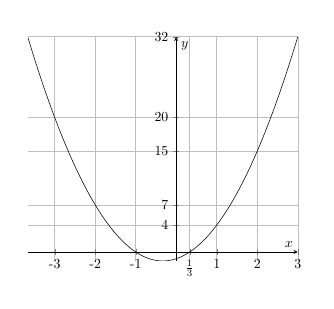
\begin{tikzpicture}[scale=0.5]
\begin{axis}[
    axis lines = middle,
    grid=major,
    legend pos={south west},
    xlabel = {$x$},
    ylabel = {$y$},
    xtick={-4, -3, -2, -1,0.333, 1,2, 3},
    xticklabels={-4,-3, -2, -1,$\frac{1}{3}$, 1,2,3},
    ytick={-5,20,7,4, 15,32},
              ]
	\addplot[domain=-3.66:3, samples=100, color=black] {3*x*x+2*x-1};
%\addplot[domain=-3.1:2.5, samples=100, color=red] {70*abs(1-2*abs(abs(x)-2))-10*x^2+10*x-70};
	%\addlegendentry{$\text{Рис. 1}$};
\end{axis}
\end{tikzpicture}$$
